\documentclass[1p]{elsarticle_modified}
%\bibliographystyle{elsarticle-num}

%\usepackage[colorlinks]{hyperref}
%\usepackage{abbrmath_seonhwa} %\Abb, \Ascr, \Acal ,\Abf, \Afrak
\usepackage{amsfonts}
\usepackage{amssymb}
\usepackage{amsmath}
\usepackage{amsthm}
\usepackage{scalefnt}
\usepackage{amsbsy}
\usepackage{kotex}
\usepackage{caption}
\usepackage{subfig}
\usepackage{color}
\usepackage{graphicx}
\usepackage{xcolor} %% white, black, red, green, blue, cyan, magenta, yellow
\usepackage{float}
\usepackage{setspace}
\usepackage{hyperref}

\usepackage{tikz}
\usetikzlibrary{arrows}

\usepackage{multirow}
\usepackage{array} % fixed length table
\usepackage{hhline}

%%%%%%%%%%%%%%%%%%%%%
\makeatletter
\renewcommand*\env@matrix[1][\arraystretch]{%
	\edef\arraystretch{#1}%
	\hskip -\arraycolsep
	\let\@ifnextchar\new@ifnextchar
	\array{*\c@MaxMatrixCols c}}
\makeatother %https://tex.stackexchange.com/questions/14071/how-can-i-increase-the-line-spacing-in-a-matrix
%%%%%%%%%%%%%%%

\usepackage[normalem]{ulem}

\newcommand{\msout}[1]{\ifmmode\text{\sout{\ensuremath{#1}}}\else\sout{#1}\fi}
%SOURCE: \msout is \stkout macro in https://tex.stackexchange.com/questions/20609/strikeout-in-math-mode

\newcommand{\cancel}[1]{
	\ifmmode
	{\color{red}\msout{#1}}
	\else
	{\color{red}\sout{#1}}
	\fi
}

\newcommand{\add}[1]{
	{\color{blue}\uwave{#1}}
}

\newcommand{\replace}[2]{
	\ifmmode
	{\color{red}\msout{#1}}{\color{blue}\uwave{#2}}
	\else
	{\color{red}\sout{#1}}{\color{blue}\uwave{#2}}
	\fi
}

\newcommand{\Sol}{\mathcal{S}} %segment
\newcommand{\D}{D} %diagram
\newcommand{\A}{\mathcal{A}} %arc


%%%%%%%%%%%%%%%%%%%%%%%%%%%%%5 test

\def\sl{\operatorname{\textup{SL}}(2,\Cbb)}
\def\psl{\operatorname{\textup{PSL}}(2,\Cbb)}
\def\quan{\mkern 1mu \triangleright \mkern 1mu}

\theoremstyle{definition}
\newtheorem{thm}{Theorem}[section]
\newtheorem{prop}[thm]{Proposition}
\newtheorem{lem}[thm]{Lemma}
\newtheorem{ques}[thm]{Question}
\newtheorem{cor}[thm]{Corollary}
\newtheorem{defn}[thm]{Definition}
\newtheorem{exam}[thm]{Example}
\newtheorem{rmk}[thm]{Remark}
\newtheorem{alg}[thm]{Algorithm}

\newcommand{\I}{\sqrt{-1}}
\begin{document}

%\begin{frontmatter}
%
%\title{Boundary parabolic representations of knots up to 8 crossings}
%
%%% Group authors per affiliation:
%\author{Yunhi Cho} 
%\address{Department of Mathematics, University of Seoul, Seoul, Korea}
%\ead{yhcho@uos.ac.kr}
%
%
%\author{Seonhwa Kim} %\fnref{s_kim}}
%\address{Center for Geometry and Physics, Institute for Basic Science, Pohang, 37673, Korea}
%\ead{ryeona17@ibs.re.kr}
%
%\author{Hyuk Kim}
%\address{Department of Mathematical Sciences, Seoul National University, Seoul 08826, Korea}
%\ead{hyukkim@snu.ac.kr}
%
%\author{Seokbeom Yoon}
%\address{Department of Mathematical Sciences, Seoul National University, Seoul, 08826,  Korea}
%\ead{sbyoon15@snu.ac.kr}
%
%\begin{abstract}
%We find all boundary parabolic representation of knots up to 8 crossings.
%
%\end{abstract}
%\begin{keyword}
%    \MSC[2010] 57M25 
%\end{keyword}
%
%\end{frontmatter}

%\linenumbers
%\tableofcontents
%
\newcommand\colored[1]{\textcolor{white}{\rule[-0.35ex]{0.8em}{1.4ex}}\kern-0.8em\color{red} #1}%
%\newcommand\colored[1]{\textcolor{white}{ #1}\kern-2.17ex	\textcolor{white}{ #1}\kern-1.81ex	\textcolor{white}{ #1}\kern-2.15ex\color{red}#1	}

{\Large $\underline{12n_{0619}~(K12n_{0619})}$}

\setlength{\tabcolsep}{10pt}
\renewcommand{\arraystretch}{1.6}
\vspace{1cm}\begin{tabular}{m{100pt}>{\centering\arraybackslash}m{274pt}}
\multirow{5}{120pt}{
	\centering
	\includegraphics[width=112pt]{../../../GIT/diagram.site/Diagrams/png/2708_12n_0619.png}\\
\ \ \ A knot diagram\footnotemark}&
\allowdisplaybreaks
\textbf{Linearized knot diagam} \\
\cline{2-2}
 &
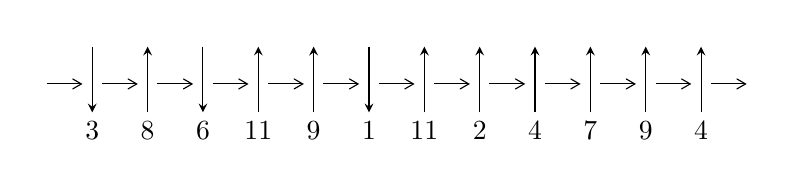
\begin{tikzpicture}[x=20pt, y=17pt]
	% nodes
	\node (C0) at (0, 0) {};
	\node (C1) at (1, 0) {};
	\node (C1U) at (1, +1) {};
	\node (C1D) at (1, -1) {3};

	\node (C2) at (2, 0) {};
	\node (C2U) at (2, +1) {};
	\node (C2D) at (2, -1) {8};

	\node (C3) at (3, 0) {};
	\node (C3U) at (3, +1) {};
	\node (C3D) at (3, -1) {6};

	\node (C4) at (4, 0) {};
	\node (C4U) at (4, +1) {};
	\node (C4D) at (4, -1) {11};

	\node (C5) at (5, 0) {};
	\node (C5U) at (5, +1) {};
	\node (C5D) at (5, -1) {9};

	\node (C6) at (6, 0) {};
	\node (C6U) at (6, +1) {};
	\node (C6D) at (6, -1) {1};

	\node (C7) at (7, 0) {};
	\node (C7U) at (7, +1) {};
	\node (C7D) at (7, -1) {11};

	\node (C8) at (8, 0) {};
	\node (C8U) at (8, +1) {};
	\node (C8D) at (8, -1) {2};

	\node (C9) at (9, 0) {};
	\node (C9U) at (9, +1) {};
	\node (C9D) at (9, -1) {4};

	\node (C10) at (10, 0) {};
	\node (C10U) at (10, +1) {};
	\node (C10D) at (10, -1) {7};

	\node (C11) at (11, 0) {};
	\node (C11U) at (11, +1) {};
	\node (C11D) at (11, -1) {9};

	\node (C12) at (12, 0) {};
	\node (C12U) at (12, +1) {};
	\node (C12D) at (12, -1) {4};
	\node (C13) at (13, 0) {};

	% arrows
	\draw[->,>={angle 60}]
	(C0) edge (C1) (C1) edge (C2) (C2) edge (C3) (C3) edge (C4) (C4) edge (C5) (C5) edge (C6) (C6) edge (C7) (C7) edge (C8) (C8) edge (C9) (C9) edge (C10) (C10) edge (C11) (C11) edge (C12) (C12) edge (C13) ;	\draw[->,>=stealth]
	(C1U) edge (C1D) (C2D) edge (C2U) (C3U) edge (C3D) (C4D) edge (C4U) (C5D) edge (C5U) (C6U) edge (C6D) (C7D) edge (C7U) (C8D) edge (C8U) (C9D) edge (C9U) (C10D) edge (C10U) (C11D) edge (C11U) (C12D) edge (C12U) ;
	\end{tikzpicture} \\
\hhline{~~} \\& 
\textbf{Solving Sequence} \\ \cline{2-2} 
 &
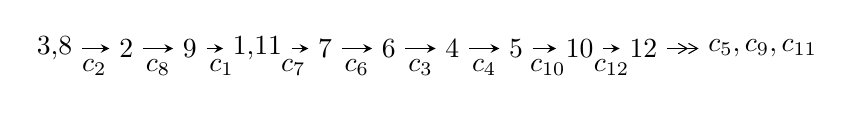
\begin{tikzpicture}[x=23pt, y=7pt]
	% node
	\node (A0) at (-1/8, 0) {3,8};
	\node (A1) at (1, 0) {2};
	\node (A2) at (2, 0) {9};
	\node (A3) at (49/16, 0) {1,11};
	\node (A4) at (33/8, 0) {7};
	\node (A5) at (41/8, 0) {6};
	\node (A6) at (49/8, 0) {4};
	\node (A7) at (57/8, 0) {5};
	\node (A8) at (65/8, 0) {10};
	\node (A9) at (73/8, 0) {12};
	\node (C1) at (1/2, -1) {$c_{2}$};
	\node (C2) at (3/2, -1) {$c_{8}$};
	\node (C3) at (5/2, -1) {$c_{1}$};
	\node (C4) at (29/8, -1) {$c_{7}$};
	\node (C5) at (37/8, -1) {$c_{6}$};
	\node (C6) at (45/8, -1) {$c_{3}$};
	\node (C7) at (53/8, -1) {$c_{4}$};
	\node (C8) at (61/8, -1) {$c_{10}$};
	\node (C9) at (69/8, -1) {$c_{12}$};
	\node (A10) at (11, 0) {$c_{5},c_{9},c_{11}$};

	% edge
	\draw[->,>=stealth]	
	(A0) edge (A1) (A1) edge (A2) (A2) edge (A3) (A3) edge (A4) (A4) edge (A5) (A5) edge (A6) (A6) edge (A7) (A7) edge (A8) (A8) edge (A9) ;
	\draw[->>,>={angle 60}]	
	(A9) edge (A10);
\end{tikzpicture} \\ 

\end{tabular} \\

\footnotetext{
The image of knot diagram is generated by the software ``\textbf{Draw programme}" developed by Andrew Bartholomew(\url{http://www.layer8.co.uk/maths/draw/index.htm\#Running-draw}), where we modified some parts for our purpose(\url{https://github.com/CATsTAILs/LinksPainter}).
}\phantom \\ \newline 
\centering \textbf{Ideals for irreducible components\footnotemark of $X_{\text{par}}$} 
 
\begin{align*}
I^u_{1}&=\langle 
4.28036\times10^{89} u^{71}+6.03330\times10^{89} u^{70}+\cdots+9.62134\times10^{90} b+1.51309\times10^{91},\\
\phantom{I^u_{1}}&\phantom{= \langle  }2.28885\times10^{91} u^{71}-3.14485\times10^{90} u^{70}+\cdots+1.25077\times10^{92} a-5.93546\times10^{92},\;u^{72}+u^{71}+\cdots-5 u+13\rangle \\
I^u_{2}&=\langle 
58306 u^{29}-92181 u^{28}+\cdots+145157 b-132553,\\
\phantom{I^u_{2}}&\phantom{= \langle  }213726 u^{29}-58787 u^{28}+\cdots+145157 a-315469,\;u^{30}+8 u^{28}+\cdots-2 u+1\rangle \\
\\
\end{align*}
\raggedright * 2 irreducible components of $\dim_{\mathbb{C}}=0$, with total 102 representations.\\
\footnotetext{All coefficients of polynomials are rational numbers. But the coefficients are sometimes approximated in decimal forms when there is not enough margin.}
\newpage
\renewcommand{\arraystretch}{1}
\centering \section*{I. $I^u_{1}= \langle 4.28\times10^{89} u^{71}+6.03\times10^{89} u^{70}+\cdots+9.62\times10^{90} b+1.51\times10^{91},\;2.29\times10^{91} u^{71}-3.14\times10^{90} u^{70}+\cdots+1.25\times10^{92} a-5.94\times10^{92},\;u^{72}+u^{71}+\cdots-5 u+13 \rangle$}
\flushleft \textbf{(i) Arc colorings}\\
\begin{tabular}{m{7pt} m{180pt} m{7pt} m{180pt} }
\flushright $a_{3}=$&$\begin{pmatrix}1\\0\end{pmatrix}$ \\
\flushright $a_{8}=$&$\begin{pmatrix}0\\u\end{pmatrix}$ \\
\flushright $a_{2}=$&$\begin{pmatrix}1\\u^2\end{pmatrix}$ \\
\flushright $a_{9}=$&$\begin{pmatrix}u\\u^3+u\end{pmatrix}$ \\
\flushright $a_{1}=$&$\begin{pmatrix}u^2+1\\u^2\end{pmatrix}$ \\
\flushright $a_{11}=$&$\begin{pmatrix}-0.182994 u^{71}+0.0251433 u^{70}+\cdots-18.8680 u+4.74543\\-0.0444882 u^{71}-0.0627074 u^{70}+\cdots+7.89374 u-1.57263\end{pmatrix}$ \\
\flushright $a_{7}=$&$\begin{pmatrix}-0.133370 u^{71}+0.0680367 u^{70}+\cdots-7.84939 u-3.40355\\-0.00317815 u^{71}+0.0974739 u^{70}+\cdots-5.89041 u+5.78176\end{pmatrix}$ \\
\flushright $a_{6}=$&$\begin{pmatrix}-0.150162 u^{71}+0.195372 u^{70}+\cdots-15.9473 u+1.82218\\-0.0760366 u^{71}+0.0252163 u^{70}+\cdots-5.90165 u+3.91591\end{pmatrix}$ \\
\flushright $a_{4}=$&$\begin{pmatrix}0.453018 u^{71}+0.167249 u^{70}+\cdots+12.8155 u-3.75646\\0.215863 u^{71}+0.311273 u^{70}+\cdots-4.36625 u+4.19897\end{pmatrix}$ \\
\flushright $a_{5}=$&$\begin{pmatrix}0.188422 u^{71}-0.0605806 u^{70}+\cdots+12.5787 u+0.355877\\-0.0375701 u^{71}+0.0536453 u^{70}+\cdots+2.51828 u-2.99277\end{pmatrix}$ \\
\flushright $a_{10}=$&$\begin{pmatrix}-0.580665 u^{71}-0.174180 u^{70}+\cdots-9.44693 u+5.13081\\-0.225939 u^{71}-0.372106 u^{70}+\cdots+10.8961 u-6.94834\end{pmatrix}$ \\
\flushright $a_{12}=$&$\begin{pmatrix}-0.215107 u^{71}-0.0246516 u^{70}+\cdots-19.2815 u+5.20660\\-0.0206372 u^{71}-0.0874849 u^{70}+\cdots+7.80928 u-0.881593\end{pmatrix}$\\&\end{tabular}
\flushleft \textbf{(ii) Obstruction class $= -1$}\\~\\
\flushleft \textbf{(iii) Cusp Shapes $= 1.23866 u^{71}+1.66942 u^{70}+\cdots+6.74520 u+28.1649$}\\~\\
\newpage\renewcommand{\arraystretch}{1}
\flushleft \textbf{(iv) u-Polynomials at the component}\newline \\
\begin{tabular}{m{50pt}|m{274pt}}
Crossings & \hspace{64pt}u-Polynomials at each crossing \\
\hline $$\begin{aligned}c_{1}\end{aligned}$$&$\begin{aligned}
&u^{72}+29 u^{71}+\cdots+1483 u+169
\end{aligned}$\\
\hline $$\begin{aligned}c_{2},c_{8}\end{aligned}$$&$\begin{aligned}
&u^{72}+u^{71}+\cdots-5 u+13
\end{aligned}$\\
\hline $$\begin{aligned}c_{3}\end{aligned}$$&$\begin{aligned}
&u^{72}-8 u^{71}+\cdots-1454 u+103
\end{aligned}$\\
\hline $$\begin{aligned}c_{4}\end{aligned}$$&$\begin{aligned}
&u^{72}-2 u^{71}+\cdots+2563738 u+372821
\end{aligned}$\\
\hline $$\begin{aligned}c_{5}\end{aligned}$$&$\begin{aligned}
&u^{72}-6 u^{71}+\cdots-62302304 u+12968512
\end{aligned}$\\
\hline $$\begin{aligned}c_{6}\end{aligned}$$&$\begin{aligned}
&u^{72}+2 u^{71}+\cdots-81136 u+4448
\end{aligned}$\\
\hline $$\begin{aligned}c_{7},c_{10}\end{aligned}$$&$\begin{aligned}
&u^{72}-3 u^{71}+\cdots-11 u-1
\end{aligned}$\\
\hline $$\begin{aligned}c_{9}\end{aligned}$$&$\begin{aligned}
&u^{72}+u^{71}+\cdots-77411 u-34673
\end{aligned}$\\
\hline $$\begin{aligned}c_{11}\end{aligned}$$&$\begin{aligned}
&u^{72}+7 u^{71}+\cdots-7376 u-2363
\end{aligned}$\\
\hline $$\begin{aligned}c_{12}\end{aligned}$$&$\begin{aligned}
&u^{72}+10 u^{71}+\cdots-582696 u-825103
\end{aligned}$\\
\hline
\end{tabular}\\~\\
\newpage\renewcommand{\arraystretch}{1}
\flushleft \textbf{(v) Riley Polynomials at the component}\newline \\
\begin{tabular}{m{50pt}|m{274pt}}
Crossings & \hspace{64pt}Riley Polynomials at each crossing \\
\hline $$\begin{aligned}c_{1}\end{aligned}$$&$\begin{aligned}
&y^{72}+41 y^{71}+\cdots-4031249 y+28561
\end{aligned}$\\
\hline $$\begin{aligned}c_{2},c_{8}\end{aligned}$$&$\begin{aligned}
&y^{72}+29 y^{71}+\cdots+1483 y+169
\end{aligned}$\\
\hline $$\begin{aligned}c_{3}\end{aligned}$$&$\begin{aligned}
&y^{72}+8 y^{71}+\cdots+86788 y+10609
\end{aligned}$\\
\hline $$\begin{aligned}c_{4}\end{aligned}$$&$\begin{aligned}
&y^{72}-108 y^{71}+\cdots-1786672638490 y+138995498041
\end{aligned}$\\
\hline $$\begin{aligned}c_{5}\end{aligned}$$&$\begin{aligned}
&y^{72}-78 y^{71}+\cdots+6347781005638656 y+168182303494144
\end{aligned}$\\
\hline $$\begin{aligned}c_{6}\end{aligned}$$&$\begin{aligned}
&y^{72}+24 y^{71}+\cdots-1766542592 y+19784704
\end{aligned}$\\
\hline $$\begin{aligned}c_{7},c_{10}\end{aligned}$$&$\begin{aligned}
&y^{72}-63 y^{71}+\cdots+91 y+1
\end{aligned}$\\
\hline $$\begin{aligned}c_{9}\end{aligned}$$&$\begin{aligned}
&y^{72}-99 y^{71}+\cdots-7903121 y+1202216929
\end{aligned}$\\
\hline $$\begin{aligned}c_{11}\end{aligned}$$&$\begin{aligned}
&y^{72}-105 y^{71}+\cdots-197872558 y+5583769
\end{aligned}$\\
\hline $$\begin{aligned}c_{12}\end{aligned}$$&$\begin{aligned}
&y^{72}-56 y^{71}+\cdots-78126375735346 y+680794960609
\end{aligned}$\\
\hline
\end{tabular}\\~\\
\newpage\flushleft \textbf{(vi) Complex Volumes and Cusp Shapes}
$$\begin{array}{c|c|c}  
\text{Solutions to }I^u_{1}& \I (\text{vol} + \sqrt{-1}CS) & \text{Cusp shape}\\
 \hline 
\begin{aligned}
u &= -0.808887 + 0.575194 I \\
a &= -0.684141 - 1.018880 I \\
b &= -1.59723 + 0.99383 I\end{aligned}
 & \phantom{-}4.62016 + 3.05851 I & \phantom{-0.000000 } 0 \\ \hline\begin{aligned}
u &= -0.808887 - 0.575194 I \\
a &= -0.684141 + 1.018880 I \\
b &= -1.59723 - 0.99383 I\end{aligned}
 & \phantom{-}4.62016 - 3.05851 I & \phantom{-0.000000 } 0 \\ \hline\begin{aligned}
u &= -0.696036 + 0.740230 I \\
a &= -0.037316 - 0.349653 I \\
b &= \phantom{-}1.31015 + 0.85715 I\end{aligned}
 & \phantom{-}6.64464 - 3.46257 I & \phantom{-0.000000 } 0 \\ \hline\begin{aligned}
u &= -0.696036 - 0.740230 I \\
a &= -0.037316 + 0.349653 I \\
b &= \phantom{-}1.31015 - 0.85715 I\end{aligned}
 & \phantom{-}6.64464 + 3.46257 I & \phantom{-0.000000 } 0 \\ \hline\begin{aligned}
u &= -0.507319 + 0.820349 I \\
a &= -1.222130 + 0.637102 I \\
b &= -0.580847 + 0.867836 I\end{aligned}
 & -3.86547 - 2.02217 I & \phantom{-}6.00000 + 0. I\phantom{ +0.000000I} \\ \hline\begin{aligned}
u &= -0.507319 - 0.820349 I \\
a &= -1.222130 - 0.637102 I \\
b &= -0.580847 - 0.867836 I\end{aligned}
 & -3.86547 + 2.02217 I & \phantom{-}6.00000 + 0. I\phantom{ +0.000000I} \\ \hline\begin{aligned}
u &= -0.116021 + 0.940603 I \\
a &= \phantom{-}0.784994 - 0.355068 I \\
b &= \phantom{-}0.65806 + 1.54944 I\end{aligned}
 & \phantom{-}2.64894 - 3.41631 I & \phantom{-}3.10260 + 2.08330 I \\ \hline\begin{aligned}
u &= -0.116021 - 0.940603 I \\
a &= \phantom{-}0.784994 + 0.355068 I \\
b &= \phantom{-}0.65806 - 1.54944 I\end{aligned}
 & \phantom{-}2.64894 + 3.41631 I & \phantom{-}3.10260 - 2.08330 I \\ \hline\begin{aligned}
u &= \phantom{-}0.673339 + 0.666930 I \\
a &= -1.09226 + 1.19514 I \\
b &= -0.87160 - 1.61399 I\end{aligned}
 & \phantom{-}11.74130 + 0.35138 I & \phantom{-}18.3982 + 2.1314 I \\ \hline\begin{aligned}
u &= \phantom{-}0.673339 - 0.666930 I \\
a &= -1.09226 - 1.19514 I \\
b &= -0.87160 + 1.61399 I\end{aligned}
 & \phantom{-}11.74130 - 0.35138 I & \phantom{-}18.3982 - 2.1314 I\\
 \hline 
 \end{array}$$\newpage$$\begin{array}{c|c|c}  
\text{Solutions to }I^u_{1}& \I (\text{vol} + \sqrt{-1}CS) & \text{Cusp shape}\\
 \hline 
\begin{aligned}
u &= -0.814321 + 0.703037 I \\
a &= \phantom{-}0.89240 + 1.61244 I \\
b &= \phantom{-}1.70285 - 0.14650 I\end{aligned}
 & \phantom{-}13.40880 + 1.35348 I & \phantom{-0.000000 } 0 \\ \hline\begin{aligned}
u &= -0.814321 - 0.703037 I \\
a &= \phantom{-}0.89240 - 1.61244 I \\
b &= \phantom{-}1.70285 + 0.14650 I\end{aligned}
 & \phantom{-}13.40880 - 1.35348 I & \phantom{-0.000000 } 0 \\ \hline\begin{aligned}
u &= \phantom{-}0.163802 + 1.063820 I \\
a &= -0.618870 + 0.559588 I \\
b &= -1.035320 - 0.100786 I\end{aligned}
 & -2.41601 + 2.16254 I & \phantom{-0.000000 } 0 \\ \hline\begin{aligned}
u &= \phantom{-}0.163802 - 1.063820 I \\
a &= -0.618870 - 0.559588 I \\
b &= -1.035320 + 0.100786 I\end{aligned}
 & -2.41601 - 2.16254 I & \phantom{-0.000000 } 0 \\ \hline\begin{aligned}
u &= \phantom{-}0.082091 + 1.074760 I \\
a &= \phantom{-}0.393708 - 1.225530 I \\
b &= \phantom{-}0.041526 - 1.307790 I\end{aligned}
 & \phantom{-}7.12176 + 1.27412 I & \phantom{-0.000000 } 0 \\ \hline\begin{aligned}
u &= \phantom{-}0.082091 - 1.074760 I \\
a &= \phantom{-}0.393708 + 1.225530 I \\
b &= \phantom{-}0.041526 + 1.307790 I\end{aligned}
 & \phantom{-}7.12176 - 1.27412 I & \phantom{-0.000000 } 0 \\ \hline\begin{aligned}
u &= -0.381326 + 0.829948 I \\
a &= \phantom{-}1.264630 - 0.364539 I \\
b &= \phantom{-}0.22348 - 1.40162 I\end{aligned}
 & -4.56914 - 1.60830 I & \phantom{-}11.92985 + 7.22454 I \\ \hline\begin{aligned}
u &= -0.381326 - 0.829948 I \\
a &= \phantom{-}1.264630 + 0.364539 I \\
b &= \phantom{-}0.22348 + 1.40162 I\end{aligned}
 & -4.56914 + 1.60830 I & \phantom{-}11.92985 - 7.22454 I \\ \hline\begin{aligned}
u &= \phantom{-}0.727539 + 0.822056 I \\
a &= -1.044260 + 0.906641 I \\
b &= -2.41732 - 0.54518 I\end{aligned}
 & \phantom{-}4.49876 - 0.62881 I & \phantom{-0.000000 } 0 \\ \hline\begin{aligned}
u &= \phantom{-}0.727539 - 0.822056 I \\
a &= -1.044260 - 0.906641 I \\
b &= -2.41732 + 0.54518 I\end{aligned}
 & \phantom{-}4.49876 + 0.62881 I & \phantom{-0.000000 } 0\\
 \hline 
 \end{array}$$\newpage$$\begin{array}{c|c|c}  
\text{Solutions to }I^u_{1}& \I (\text{vol} + \sqrt{-1}CS) & \text{Cusp shape}\\
 \hline 
\begin{aligned}
u &= \phantom{-}0.787450 + 0.775531 I \\
a &= -0.77260 - 1.30907 I \\
b &= -0.086400 - 1.042150 I\end{aligned}
 & \phantom{-}8.46954 - 2.16031 I & \phantom{-0.000000 } 0 \\ \hline\begin{aligned}
u &= \phantom{-}0.787450 - 0.775531 I \\
a &= -0.77260 + 1.30907 I \\
b &= -0.086400 + 1.042150 I\end{aligned}
 & \phantom{-}8.46954 + 2.16031 I & \phantom{-0.000000 } 0 \\ \hline\begin{aligned}
u &= -0.707731 + 0.849293 I \\
a &= -0.453970 - 1.024470 I \\
b &= -1.43457 + 0.83997 I\end{aligned}
 & \phantom{-}4.40743 - 0.27804 I & \phantom{-0.000000 } 0 \\ \hline\begin{aligned}
u &= -0.707731 - 0.849293 I \\
a &= -0.453970 + 1.024470 I \\
b &= -1.43457 - 0.83997 I\end{aligned}
 & \phantom{-}4.40743 + 0.27804 I & \phantom{-0.000000 } 0 \\ \hline\begin{aligned}
u &= -0.703670 + 0.875856 I \\
a &= \phantom{-}0.974104 + 0.503213 I \\
b &= \phantom{-}2.34182 - 0.65068 I\end{aligned}
 & \phantom{-}4.32813 - 5.13090 I & \phantom{-0.000000 } 0 \\ \hline\begin{aligned}
u &= -0.703670 - 0.875856 I \\
a &= \phantom{-}0.974104 - 0.503213 I \\
b &= \phantom{-}2.34182 + 0.65068 I\end{aligned}
 & \phantom{-}4.32813 + 5.13090 I & \phantom{-0.000000 } 0 \\ \hline\begin{aligned}
u &= \phantom{-}0.909432 + 0.660037 I \\
a &= \phantom{-}1.199680 - 0.671979 I \\
b &= \phantom{-}1.87323 + 0.59826 I\end{aligned}
 & \phantom{-}5.55068 - 0.89067 I & \phantom{-0.000000 } 0 \\ \hline\begin{aligned}
u &= \phantom{-}0.909432 - 0.660037 I \\
a &= \phantom{-}1.199680 + 0.671979 I \\
b &= \phantom{-}1.87323 - 0.59826 I\end{aligned}
 & \phantom{-}5.55068 + 0.89067 I & \phantom{-0.000000 } 0 \\ \hline\begin{aligned}
u &= \phantom{-}0.638035 + 0.594328 I \\
a &= \phantom{-}0.489358 + 0.549201 I \\
b &= \phantom{-}0.153674 + 0.397027 I\end{aligned}
 & \phantom{-}1.46159 + 0.94369 I & \phantom{-}8.05381 - 3.32759 I \\ \hline\begin{aligned}
u &= \phantom{-}0.638035 - 0.594328 I \\
a &= \phantom{-}0.489358 - 0.549201 I \\
b &= \phantom{-}0.153674 - 0.397027 I\end{aligned}
 & \phantom{-}1.46159 - 0.94369 I & \phantom{-}8.05381 + 3.32759 I\\
 \hline 
 \end{array}$$\newpage$$\begin{array}{c|c|c}  
\text{Solutions to }I^u_{1}& \I (\text{vol} + \sqrt{-1}CS) & \text{Cusp shape}\\
 \hline 
\begin{aligned}
u &= -0.292414 + 1.099760 I \\
a &= -0.045977 + 0.161008 I \\
b &= -0.183182 - 0.301441 I\end{aligned}
 & -3.74250 - 0.35528 I & \phantom{-0.000000 } 0 \\ \hline\begin{aligned}
u &= -0.292414 - 1.099760 I \\
a &= -0.045977 - 0.161008 I \\
b &= -0.183182 + 0.301441 I\end{aligned}
 & -3.74250 + 0.35528 I & \phantom{-0.000000 } 0 \\ \hline\begin{aligned}
u &= \phantom{-}0.711303 + 0.912423 I \\
a &= \phantom{-}0.868327 - 1.090420 I \\
b &= \phantom{-}2.09993 + 0.93166 I\end{aligned}
 & \phantom{-}4.21886 + 6.12406 I & \phantom{-0.000000 } 0 \\ \hline\begin{aligned}
u &= \phantom{-}0.711303 - 0.912423 I \\
a &= \phantom{-}0.868327 + 1.090420 I \\
b &= \phantom{-}2.09993 - 0.93166 I\end{aligned}
 & \phantom{-}4.21886 - 6.12406 I & \phantom{-0.000000 } 0 \\ \hline\begin{aligned}
u &= \phantom{-}0.594374 + 1.009220 I \\
a &= \phantom{-}0.509259 + 0.475060 I \\
b &= \phantom{-}0.236822 + 0.688574 I\end{aligned}
 & \phantom{-}0.20929 + 3.90599 I & \phantom{-0.000000 } 0 \\ \hline\begin{aligned}
u &= \phantom{-}0.594374 - 1.009220 I \\
a &= \phantom{-}0.509259 - 0.475060 I \\
b &= \phantom{-}0.236822 - 0.688574 I\end{aligned}
 & \phantom{-}0.20929 - 3.90599 I & \phantom{-0.000000 } 0 \\ \hline\begin{aligned}
u &= \phantom{-}0.034956 + 0.821119 I \\
a &= -0.41604 - 1.41541 I \\
b &= -0.161306 + 0.517047 I\end{aligned}
 & \phantom{-}0.25599 - 2.44516 I & \phantom{-}3.51232 + 3.05197 I \\ \hline\begin{aligned}
u &= \phantom{-}0.034956 - 0.821119 I \\
a &= -0.41604 + 1.41541 I \\
b &= -0.161306 - 0.517047 I\end{aligned}
 & \phantom{-}0.25599 + 2.44516 I & \phantom{-}3.51232 - 3.05197 I \\ \hline\begin{aligned}
u &= -1.013690 + 0.601362 I \\
a &= \phantom{-}0.99520 + 1.11698 I \\
b &= \phantom{-}1.73415 - 0.41392 I\end{aligned}
 & \phantom{-}15.2060 + 9.6384 I & \phantom{-0.000000 } 0 \\ \hline\begin{aligned}
u &= -1.013690 - 0.601362 I \\
a &= \phantom{-}0.99520 - 1.11698 I \\
b &= \phantom{-}1.73415 + 0.41392 I\end{aligned}
 & \phantom{-}15.2060 - 9.6384 I & \phantom{-0.000000 } 0\\
 \hline 
 \end{array}$$\newpage$$\begin{array}{c|c|c}  
\text{Solutions to }I^u_{1}& \I (\text{vol} + \sqrt{-1}CS) & \text{Cusp shape}\\
 \hline 
\begin{aligned}
u &= -0.677870 + 0.977881 I \\
a &= \phantom{-}0.213548 - 0.199030 I \\
b &= \phantom{-}0.580098 + 1.130410 I\end{aligned}
 & \phantom{-}5.90968 - 1.84580 I & \phantom{-0.000000 } 0 \\ \hline\begin{aligned}
u &= -0.677870 - 0.977881 I \\
a &= \phantom{-}0.213548 + 0.199030 I \\
b &= \phantom{-}0.580098 - 1.130410 I\end{aligned}
 & \phantom{-}5.90968 + 1.84580 I & \phantom{-0.000000 } 0 \\ \hline\begin{aligned}
u &= \phantom{-}0.655258 + 1.004640 I \\
a &= \phantom{-}0.723304 - 0.915460 I \\
b &= \phantom{-}2.78885 - 0.55758 I\end{aligned}
 & \phantom{-}10.71060 + 4.84302 I & \phantom{-0.000000 } 0 \\ \hline\begin{aligned}
u &= \phantom{-}0.655258 - 1.004640 I \\
a &= \phantom{-}0.723304 + 0.915460 I \\
b &= \phantom{-}2.78885 + 0.55758 I\end{aligned}
 & \phantom{-}10.71060 - 4.84302 I & \phantom{-0.000000 } 0 \\ \hline\begin{aligned}
u &= \phantom{-}0.738710 + 0.963164 I \\
a &= -1.19204 - 0.78105 I \\
b &= -0.675198 - 1.198490 I\end{aligned}
 & \phantom{-}7.89130 + 7.92115 I & \phantom{-0.000000 } 0 \\ \hline\begin{aligned}
u &= \phantom{-}0.738710 - 0.963164 I \\
a &= -1.19204 + 0.78105 I \\
b &= -0.675198 + 1.198490 I\end{aligned}
 & \phantom{-}7.89130 - 7.92115 I & \phantom{-0.000000 } 0 \\ \hline\begin{aligned}
u &= \phantom{-}1.144690 + 0.425981 I \\
a &= -1.218740 + 0.443843 I \\
b &= -1.52526 - 0.51644 I\end{aligned}
 & \phantom{-}13.72910 + 2.93341 I & \phantom{-0.000000 } 0 \\ \hline\begin{aligned}
u &= \phantom{-}1.144690 - 0.425981 I \\
a &= -1.218740 - 0.443843 I \\
b &= -1.52526 + 0.51644 I\end{aligned}
 & \phantom{-}13.72910 - 2.93341 I & \phantom{-0.000000 } 0 \\ \hline\begin{aligned}
u &= -0.550235 + 1.099390 I \\
a &= -0.0754485 + 0.0197779 I \\
b &= \phantom{-}0.160032 - 0.367219 I\end{aligned}
 & -1.98390 - 7.01272 I & \phantom{-0.000000 } 0 \\ \hline\begin{aligned}
u &= -0.550235 - 1.099390 I \\
a &= -0.0754485 - 0.0197779 I \\
b &= \phantom{-}0.160032 + 0.367219 I\end{aligned}
 & -1.98390 + 7.01272 I & \phantom{-0.000000 } 0\\
 \hline 
 \end{array}$$\newpage$$\begin{array}{c|c|c}  
\text{Solutions to }I^u_{1}& \I (\text{vol} + \sqrt{-1}CS) & \text{Cusp shape}\\
 \hline 
\begin{aligned}
u &= -0.731363 + 1.014090 I \\
a &= -1.37318 - 0.69630 I \\
b &= -2.48364 + 0.63785 I\end{aligned}
 & \phantom{-}12.4616 - 7.1678 I & \phantom{-0.000000 } 0 \\ \hline\begin{aligned}
u &= -0.731363 - 1.014090 I \\
a &= -1.37318 + 0.69630 I \\
b &= -2.48364 - 0.63785 I\end{aligned}
 & \phantom{-}12.4616 + 7.1678 I & \phantom{-0.000000 } 0 \\ \hline\begin{aligned}
u &= -0.697806 + 1.047480 I \\
a &= \phantom{-}0.861122 + 0.565843 I \\
b &= \phantom{-}2.63010 - 0.99051 I\end{aligned}
 & \phantom{-}3.25158 - 8.71682 I & \phantom{-0.000000 } 0 \\ \hline\begin{aligned}
u &= -0.697806 - 1.047480 I \\
a &= \phantom{-}0.861122 - 0.565843 I \\
b &= \phantom{-}2.63010 + 0.99051 I\end{aligned}
 & \phantom{-}3.25158 + 8.71682 I & \phantom{-0.000000 } 0 \\ \hline\begin{aligned}
u &= -0.655934 + 0.321949 I \\
a &= \phantom{-}0.195232 + 0.043457 I \\
b &= -0.292662 + 0.217665 I\end{aligned}
 & \phantom{-}0.19630 + 2.31331 I & \phantom{-}2.50410 - 3.87759 I \\ \hline\begin{aligned}
u &= -0.655934 - 0.321949 I \\
a &= \phantom{-}0.195232 - 0.043457 I \\
b &= -0.292662 - 0.217665 I\end{aligned}
 & \phantom{-}0.19630 - 2.31331 I & \phantom{-}2.50410 + 3.87759 I \\ \hline\begin{aligned}
u &= \phantom{-}0.764755 + 1.056800 I \\
a &= -0.768111 + 0.967366 I \\
b &= -2.03014 - 0.43609 I\end{aligned}
 & \phantom{-}4.34565 + 7.06034 I & \phantom{-0.000000 } 0 \\ \hline\begin{aligned}
u &= \phantom{-}0.764755 - 1.056800 I \\
a &= -0.768111 - 0.967366 I \\
b &= -2.03014 + 0.43609 I\end{aligned}
 & \phantom{-}4.34565 - 7.06034 I & \phantom{-0.000000 } 0 \\ \hline\begin{aligned}
u &= -0.078514 + 0.637068 I \\
a &= -0.140949 + 1.209800 I \\
b &= -0.473595 + 1.195070 I\end{aligned}
 & \phantom{-}0.91968 + 2.40413 I & -0.54237 - 2.15079 I \\ \hline\begin{aligned}
u &= -0.078514 - 0.637068 I \\
a &= -0.140949 - 1.209800 I \\
b &= -0.473595 - 1.195070 I\end{aligned}
 & \phantom{-}0.91968 - 2.40413 I & -0.54237 + 2.15079 I\\
 \hline 
 \end{array}$$\newpage$$\begin{array}{c|c|c}  
\text{Solutions to }I^u_{1}& \I (\text{vol} + \sqrt{-1}CS) & \text{Cusp shape}\\
 \hline 
\begin{aligned}
u &= -0.764358 + 1.130520 I \\
a &= -1.077160 - 0.723013 I \\
b &= -2.58282 + 0.58816 I\end{aligned}
 & \phantom{-}13.5431 - 16.0927 I & \phantom{-0.000000 } 0 \\ \hline\begin{aligned}
u &= -0.764358 - 1.130520 I \\
a &= -1.077160 + 0.723013 I \\
b &= -2.58282 - 0.58816 I\end{aligned}
 & \phantom{-}13.5431 + 16.0927 I & \phantom{-0.000000 } 0 \\ \hline\begin{aligned}
u &= -0.027747 + 1.400220 I \\
a &= -0.174463 + 0.765705 I \\
b &= -0.608195 - 0.323463 I\end{aligned}
 & -2.16290 + 0.96975 I & \phantom{-0.000000 } 0 \\ \hline\begin{aligned}
u &= -0.027747 - 1.400220 I \\
a &= -0.174463 - 0.765705 I \\
b &= -0.608195 + 0.323463 I\end{aligned}
 & -2.16290 - 0.96975 I & \phantom{-0.000000 } 0 \\ \hline\begin{aligned}
u &= \phantom{-}0.157578 + 1.394680 I \\
a &= \phantom{-}0.323172 - 0.990570 I \\
b &= \phantom{-}0.505882 - 0.267746 I\end{aligned}
 & \phantom{-}6.98353 + 7.23116 I & \phantom{-0.000000 } 0 \\ \hline\begin{aligned}
u &= \phantom{-}0.157578 - 1.394680 I \\
a &= \phantom{-}0.323172 + 0.990570 I \\
b &= \phantom{-}0.505882 + 0.267746 I\end{aligned}
 & \phantom{-}6.98353 - 7.23116 I & \phantom{-0.000000 } 0 \\ \hline\begin{aligned}
u &= \phantom{-}0.77726 + 1.28992 I \\
a &= \phantom{-}0.610495 - 0.781522 I \\
b &= \phantom{-}1.87938 + 0.13816 I\end{aligned}
 & \phantom{-}11.07580 + 3.96205 I & \phantom{-0.000000 } 0 \\ \hline\begin{aligned}
u &= \phantom{-}0.77726 - 1.28992 I \\
a &= \phantom{-}0.610495 + 0.781522 I \\
b &= \phantom{-}1.87938 - 0.13816 I\end{aligned}
 & \phantom{-}11.07580 - 3.96205 I & \phantom{-0.000000 } 0 \\ \hline\begin{aligned}
u &= -0.203804 + 0.401097 I \\
a &= \phantom{-}0.29924 - 1.98542 I \\
b &= \phantom{-}0.28052 + 2.03618 I\end{aligned}
 & \phantom{-}4.74098 + 2.25423 I & \phantom{-}11.54945 - 5.18126 I \\ \hline\begin{aligned}
u &= -0.203804 - 0.401097 I \\
a &= \phantom{-}0.29924 + 1.98542 I \\
b &= \phantom{-}0.28052 - 2.03618 I\end{aligned}
 & \phantom{-}4.74098 - 2.25423 I & \phantom{-}11.54945 + 5.18126 I\\
 \hline 
 \end{array}$$\newpage$$\begin{array}{c|c|c}  
\text{Solutions to }I^u_{1}& \I (\text{vol} + \sqrt{-1}CS) & \text{Cusp shape}\\
 \hline 
\begin{aligned}
u &= \phantom{-}0.444431\phantom{ +0.000000I} \\
a &= \phantom{-}1.32156\phantom{ +0.000000I} \\
b &= \phantom{-}0.457135\phantom{ +0.000000I}\end{aligned}
 & \phantom{-}0.813147\phantom{ +0.000000I} & \phantom{-}12.3290\phantom{ +0.000000I} \\ \hline\begin{aligned}
u &= \phantom{-}0.292517\phantom{ +0.000000I} \\
a &= -5.77870\phantom{ +0.000000I} \\
b &= \phantom{-}0.220364\phantom{ +0.000000I}\end{aligned}
 & \phantom{-}10.8708\phantom{ +0.000000I} & \phantom{-}3.55680\phantom{ +0.000000I}\\
 \hline 
 \end{array}$$\newpage\newpage\renewcommand{\arraystretch}{1}
\centering \section*{II. $I^u_{2}= \langle 58306 u^{29}-92181 u^{28}+\cdots+145157 b-132553,\;2.14\times10^{5} u^{29}-5.88\times10^{4} u^{28}+\cdots+1.45\times10^{5} a-3.15\times10^{5},\;u^{30}+8 u^{28}+\cdots-2 u+1 \rangle$}
\flushleft \textbf{(i) Arc colorings}\\
\begin{tabular}{m{7pt} m{180pt} m{7pt} m{180pt} }
\flushright $a_{3}=$&$\begin{pmatrix}1\\0\end{pmatrix}$ \\
\flushright $a_{8}=$&$\begin{pmatrix}0\\u\end{pmatrix}$ \\
\flushright $a_{2}=$&$\begin{pmatrix}1\\u^2\end{pmatrix}$ \\
\flushright $a_{9}=$&$\begin{pmatrix}u\\u^3+u\end{pmatrix}$ \\
\flushright $a_{1}=$&$\begin{pmatrix}u^2+1\\u^2\end{pmatrix}$ \\
\flushright $a_{11}=$&$\begin{pmatrix}-1.47238 u^{29}+0.404989 u^{28}+\cdots-12.9692 u+2.17330\\-0.401675 u^{29}+0.635043 u^{28}+\cdots-6.12894 u+0.913170\end{pmatrix}$ \\
\flushright $a_{7}=$&$\begin{pmatrix}2.01653 u^{29}-0.240560 u^{28}+\cdots+10.3514 u-0.616808\\0.712808 u^{29}+0.388531 u^{28}+\cdots+1.99596 u+0.773955\end{pmatrix}$ \\
\flushright $a_{6}=$&$\begin{pmatrix}2.55462 u^{29}+0.167591 u^{28}+\cdots+14.9088 u-1.00973\\0.174852 u^{29}+0.258892 u^{28}+\cdots+1.99550 u+0.236165\end{pmatrix}$ \\
\flushright $a_{4}=$&$\begin{pmatrix}1.70447 u^{29}-0.769353 u^{28}+\cdots+14.5271 u-5.00674\\0.230351 u^{29}-1.65192 u^{28}+\cdots+5.14174 u-2.38759\end{pmatrix}$ \\
\flushright $a_{5}=$&$\begin{pmatrix}2.31155 u^{29}-0.307440 u^{28}+\cdots+13.6258 u-0.778295\\0.377440 u^{29}+0.00674442 u^{28}+\cdots+0.00549750 u+0.942635\end{pmatrix}$ \\
\flushright $a_{10}=$&$\begin{pmatrix}1.03500 u^{29}+1.30748 u^{28}+\cdots-3.08951 u+2.26109\\0.186770 u^{29}-0.118678 u^{28}+\cdots+0.707145 u-0.350117\end{pmatrix}$ \\
\flushright $a_{12}=$&$\begin{pmatrix}-2.01033 u^{29}+0.275350 u^{28}+\cdots-12.9696 u+1.63551\\-0.889272 u^{29}+0.343531 u^{28}+\cdots-5.85073 u+0.505019\end{pmatrix}$\\&\end{tabular}
\flushleft \textbf{(ii) Obstruction class $= 1$}\\~\\
\flushleft \textbf{(iii) Cusp Shapes $= \frac{1400610}{145157} u^{29}+\frac{939828}{145157} u^{28}+\cdots+\frac{3223212}{145157} u+\frac{2462379}{145157}$}\\~\\
\newpage\renewcommand{\arraystretch}{1}
\flushleft \textbf{(iv) u-Polynomials at the component}\newline \\
\begin{tabular}{m{50pt}|m{274pt}}
Crossings & \hspace{64pt}u-Polynomials at each crossing \\
\hline $$\begin{aligned}c_{1}\end{aligned}$$&$\begin{aligned}
&u^{30}-16 u^{29}+\cdots-18 u+1
\end{aligned}$\\
\hline $$\begin{aligned}c_{2}\end{aligned}$$&$\begin{aligned}
&u^{30}+8 u^{28}+\cdots-2 u+1
\end{aligned}$\\
\hline $$\begin{aligned}c_{3}\end{aligned}$$&$\begin{aligned}
&u^{30}-11 u^{29}+\cdots-3 u+1
\end{aligned}$\\
\hline $$\begin{aligned}c_{4}\end{aligned}$$&$\begin{aligned}
&u^{30}+u^{29}+\cdots+25 u+13
\end{aligned}$\\
\hline $$\begin{aligned}c_{5}\end{aligned}$$&$\begin{aligned}
&u^{30}+3 u^{29}+\cdots-104 u+16
\end{aligned}$\\
\hline $$\begin{aligned}c_{6}\end{aligned}$$&$\begin{aligned}
&u^{30}- u^{29}+\cdots-84 u+8
\end{aligned}$\\
\hline $$\begin{aligned}c_{7}\end{aligned}$$&$\begin{aligned}
&u^{30}-2 u^{29}+\cdots-2 u+1
\end{aligned}$\\
\hline $$\begin{aligned}c_{8}\end{aligned}$$&$\begin{aligned}
&u^{30}+8 u^{28}+\cdots+2 u+1
\end{aligned}$\\
\hline $$\begin{aligned}c_{9}\end{aligned}$$&$\begin{aligned}
&u^{30}-8 u^{28}+\cdots-4 u+1
\end{aligned}$\\
\hline $$\begin{aligned}c_{10}\end{aligned}$$&$\begin{aligned}
&u^{30}+2 u^{29}+\cdots+2 u+1
\end{aligned}$\\
\hline $$\begin{aligned}c_{11}\end{aligned}$$&$\begin{aligned}
&u^{30}-14 u^{29}+\cdots-599 u+77
\end{aligned}$\\
\hline $$\begin{aligned}c_{12}\end{aligned}$$&$\begin{aligned}
&u^{30}-5 u^{29}+\cdots- u+1
\end{aligned}$\\
\hline
\end{tabular}\\~\\
\newpage\renewcommand{\arraystretch}{1}
\flushleft \textbf{(v) Riley Polynomials at the component}\newline \\
\begin{tabular}{m{50pt}|m{274pt}}
Crossings & \hspace{64pt}Riley Polynomials at each crossing \\
\hline $$\begin{aligned}c_{1}\end{aligned}$$&$\begin{aligned}
&y^{30}+8 y^{29}+\cdots-54 y+1
\end{aligned}$\\
\hline $$\begin{aligned}c_{2},c_{8}\end{aligned}$$&$\begin{aligned}
&y^{30}+16 y^{29}+\cdots+18 y+1
\end{aligned}$\\
\hline $$\begin{aligned}c_{3}\end{aligned}$$&$\begin{aligned}
&y^{30}-5 y^{29}+\cdots-9 y+1
\end{aligned}$\\
\hline $$\begin{aligned}c_{4}\end{aligned}$$&$\begin{aligned}
&y^{30}-21 y^{29}+\cdots+1533 y+169
\end{aligned}$\\
\hline $$\begin{aligned}c_{5}\end{aligned}$$&$\begin{aligned}
&y^{30}-23 y^{29}+\cdots-3520 y+256
\end{aligned}$\\
\hline $$\begin{aligned}c_{6}\end{aligned}$$&$\begin{aligned}
&y^{30}- y^{29}+\cdots-1104 y+64
\end{aligned}$\\
\hline $$\begin{aligned}c_{7},c_{10}\end{aligned}$$&$\begin{aligned}
&y^{30}-16 y^{29}+\cdots-18 y+1
\end{aligned}$\\
\hline $$\begin{aligned}c_{9}\end{aligned}$$&$\begin{aligned}
&y^{30}-16 y^{29}+\cdots+10 y+1
\end{aligned}$\\
\hline $$\begin{aligned}c_{11}\end{aligned}$$&$\begin{aligned}
&y^{30}-38 y^{29}+\cdots-117791 y+5929
\end{aligned}$\\
\hline $$\begin{aligned}c_{12}\end{aligned}$$&$\begin{aligned}
&y^{30}-13 y^{29}+\cdots+17 y+1
\end{aligned}$\\
\hline
\end{tabular}\\~\\
\newpage\flushleft \textbf{(vi) Complex Volumes and Cusp Shapes}
$$\begin{array}{c|c|c}  
\text{Solutions to }I^u_{2}& \I (\text{vol} + \sqrt{-1}CS) & \text{Cusp shape}\\
 \hline 
\begin{aligned}
u &= -0.783418 + 0.632894 I \\
a &= -0.810991 - 1.018060 I \\
b &= -1.83940 + 0.78866 I\end{aligned}
 & \phantom{-}3.40622 + 3.06203 I & \phantom{-}7.45974 - 2.51576 I \\ \hline\begin{aligned}
u &= -0.783418 - 0.632894 I \\
a &= -0.810991 + 1.018060 I \\
b &= -1.83940 - 0.78866 I\end{aligned}
 & \phantom{-}3.40622 - 3.06203 I & \phantom{-}7.45974 + 2.51576 I \\ \hline\begin{aligned}
u &= \phantom{-}0.619760 + 0.865626 I \\
a &= \phantom{-}1.16399 + 0.94071 I \\
b &= \phantom{-}0.309140 + 1.239140 I\end{aligned}
 & -3.19194 + 2.43189 I & \phantom{-}12.01531 - 5.52437 I \\ \hline\begin{aligned}
u &= \phantom{-}0.619760 - 0.865626 I \\
a &= \phantom{-}1.16399 - 0.94071 I \\
b &= \phantom{-}0.309140 - 1.239140 I\end{aligned}
 & -3.19194 - 2.43189 I & \phantom{-}12.01531 + 5.52437 I \\ \hline\begin{aligned}
u &= -0.368581 + 1.000170 I \\
a &= -0.426345 - 0.302191 I \\
b &= \phantom{-}0.67189 + 1.63285 I\end{aligned}
 & \phantom{-}3.60668 - 4.39482 I & \phantom{-}9.00853 + 6.46321 I \\ \hline\begin{aligned}
u &= -0.368581 - 1.000170 I \\
a &= -0.426345 + 0.302191 I \\
b &= \phantom{-}0.67189 - 1.63285 I\end{aligned}
 & \phantom{-}3.60668 + 4.39482 I & \phantom{-}9.00853 - 6.46321 I \\ \hline\begin{aligned}
u &= \phantom{-}0.332552 + 0.864602 I \\
a &= -1.206910 - 0.245260 I \\
b &= -0.413045 - 1.160100 I\end{aligned}
 & -4.89037 + 1.43366 I & -8.45611 + 3.24752 I \\ \hline\begin{aligned}
u &= \phantom{-}0.332552 - 0.864602 I \\
a &= -1.206910 + 0.245260 I \\
b &= -0.413045 + 1.160100 I\end{aligned}
 & -4.89037 - 1.43366 I & -8.45611 - 3.24752 I \\ \hline\begin{aligned}
u &= -0.684283 + 0.854673 I \\
a &= \phantom{-}0.818321 + 0.115887 I \\
b &= \phantom{-}2.27305 + 0.07664 I\end{aligned}
 & \phantom{-}6.45076 - 4.59120 I & \phantom{-}11.56923 + 7.10771 I \\ \hline\begin{aligned}
u &= -0.684283 - 0.854673 I \\
a &= \phantom{-}0.818321 - 0.115887 I \\
b &= \phantom{-}2.27305 - 0.07664 I\end{aligned}
 & \phantom{-}6.45076 + 4.59120 I & \phantom{-}11.56923 - 7.10771 I\\
 \hline 
 \end{array}$$\newpage$$\begin{array}{c|c|c}  
\text{Solutions to }I^u_{2}& \I (\text{vol} + \sqrt{-1}CS) & \text{Cusp shape}\\
 \hline 
\begin{aligned}
u &= -0.335307 + 0.788308 I \\
a &= -0.308397 + 0.642481 I \\
b &= \phantom{-}0.30926 + 2.50864 I\end{aligned}
 & \phantom{-}4.40509 + 1.42170 I & \phantom{-}7.66101 + 2.26727 I \\ \hline\begin{aligned}
u &= -0.335307 - 0.788308 I \\
a &= -0.308397 - 0.642481 I \\
b &= \phantom{-}0.30926 - 2.50864 I\end{aligned}
 & \phantom{-}4.40509 - 1.42170 I & \phantom{-}7.66101 - 2.26727 I \\ \hline\begin{aligned}
u &= -0.725614 + 0.892152 I \\
a &= -0.091508 - 0.819126 I \\
b &= -0.476611 + 1.081330 I\end{aligned}
 & \phantom{-}6.34146 - 0.80394 I & \phantom{-}13.14765 - 1.03633 I \\ \hline\begin{aligned}
u &= -0.725614 - 0.892152 I \\
a &= -0.091508 + 0.819126 I \\
b &= -0.476611 - 1.081330 I\end{aligned}
 & \phantom{-}6.34146 + 0.80394 I & \phantom{-}13.14765 + 1.03633 I \\ \hline\begin{aligned}
u &= \phantom{-}0.582986 + 0.610428 I \\
a &= -1.23889 + 1.49928 I \\
b &= -0.75129 - 1.21355 I\end{aligned}
 & \phantom{-}11.28510 + 0.73508 I & \phantom{-}7.51796 - 7.30910 I \\ \hline\begin{aligned}
u &= \phantom{-}0.582986 - 0.610428 I \\
a &= -1.23889 - 1.49928 I \\
b &= -0.75129 + 1.21355 I\end{aligned}
 & \phantom{-}11.28510 - 0.73508 I & \phantom{-}7.51796 + 7.30910 I \\ \hline\begin{aligned}
u &= \phantom{-}0.255399 + 1.222230 I \\
a &= -0.324792 + 0.567201 I \\
b &= -0.847986 + 0.110219 I\end{aligned}
 & -3.30623 + 1.15332 I & \phantom{-}4.33144 - 1.27674 I \\ \hline\begin{aligned}
u &= \phantom{-}0.255399 - 1.222230 I \\
a &= -0.324792 - 0.567201 I \\
b &= -0.847986 - 0.110219 I\end{aligned}
 & -3.30623 - 1.15332 I & \phantom{-}4.33144 + 1.27674 I \\ \hline\begin{aligned}
u &= \phantom{-}0.540675 + 1.125620 I \\
a &= -0.222231 + 0.444877 I \\
b &= -0.534770 + 0.403381 I\end{aligned}
 & -1.49594 + 7.00148 I & \phantom{-}12.8281 - 7.0248 I \\ \hline\begin{aligned}
u &= \phantom{-}0.540675 - 1.125620 I \\
a &= -0.222231 - 0.444877 I \\
b &= -0.534770 - 0.403381 I\end{aligned}
 & -1.49594 - 7.00148 I & \phantom{-}12.8281 + 7.0248 I\\
 \hline 
 \end{array}$$\newpage$$\begin{array}{c|c|c}  
\text{Solutions to }I^u_{2}& \I (\text{vol} + \sqrt{-1}CS) & \text{Cusp shape}\\
 \hline 
\begin{aligned}
u &= -0.700718 + 1.037000 I \\
a &= \phantom{-}0.874088 + 0.682487 I \\
b &= \phantom{-}2.43000 - 0.94490 I\end{aligned}
 & \phantom{-}2.19546 - 8.69208 I & \phantom{-}4.75207 + 7.00700 I \\ \hline\begin{aligned}
u &= -0.700718 - 1.037000 I \\
a &= \phantom{-}0.874088 - 0.682487 I \\
b &= \phantom{-}2.43000 + 0.94490 I\end{aligned}
 & \phantom{-}2.19546 + 8.69208 I & \phantom{-}4.75207 - 7.00700 I \\ \hline\begin{aligned}
u &= \phantom{-}0.711976 + 0.189161 I \\
a &= \phantom{-}1.061860 - 0.269522 I \\
b &= \phantom{-}0.438542 - 0.183348 I\end{aligned}
 & \phantom{-}1.04863 - 2.30351 I & \phantom{-}12.72741 + 3.19180 I \\ \hline\begin{aligned}
u &= \phantom{-}0.711976 - 0.189161 I \\
a &= \phantom{-}1.061860 + 0.269522 I \\
b &= \phantom{-}0.438542 + 0.183348 I\end{aligned}
 & \phantom{-}1.04863 + 2.30351 I & \phantom{-}12.72741 - 3.19180 I \\ \hline\begin{aligned}
u &= \phantom{-}0.640934 + 1.118050 I \\
a &= \phantom{-}0.700059 - 0.901785 I \\
b &= \phantom{-}2.11090 - 0.28974 I\end{aligned}
 & \phantom{-}9.61448 + 4.20198 I & \phantom{-}7.63729 - 2.59179 I \\ \hline\begin{aligned}
u &= \phantom{-}0.640934 - 1.118050 I \\
a &= \phantom{-}0.700059 + 0.901785 I \\
b &= \phantom{-}2.11090 + 0.28974 I\end{aligned}
 & \phantom{-}9.61448 - 4.20198 I & \phantom{-}7.63729 + 2.59179 I \\ \hline\begin{aligned}
u &= -0.127172 + 1.326790 I \\
a &= -0.146586 + 0.798852 I \\
b &= -0.384493 - 0.315318 I\end{aligned}
 & -2.41141 + 1.33974 I & \phantom{-}3.46635 - 9.18297 I \\ \hline\begin{aligned}
u &= -0.127172 - 1.326790 I \\
a &= -0.146586 - 0.798852 I \\
b &= -0.384493 + 0.315318 I\end{aligned}
 & -2.41141 - 1.33974 I & \phantom{-}3.46635 + 9.18297 I \\ \hline\begin{aligned}
u &= \phantom{-}0.040810 + 0.418157 I \\
a &= -0.34166 - 2.28175 I \\
b &= -0.295186 - 0.743488 I\end{aligned}
 & \phantom{-}1.48560 - 2.52463 I & \phantom{-}14.3340 + 4.6539 I \\ \hline\begin{aligned}
u &= \phantom{-}0.040810 - 0.418157 I \\
a &= -0.34166 + 2.28175 I \\
b &= -0.295186 + 0.743488 I\end{aligned}
 & \phantom{-}1.48560 + 2.52463 I & \phantom{-}14.3340 - 4.6539 I\\
 \hline 
 \end{array}$$\newpage
\newpage\renewcommand{\arraystretch}{1}
\centering \section*{ III. u-Polynomials}
\begin{tabular}{m{50pt}|m{274pt}}
Crossings & \hspace{64pt}u-Polynomials at each crossing \\
\hline $$\begin{aligned}c_{1}\end{aligned}$$&$\begin{aligned}
&(u^{30}-16 u^{29}+\cdots-18 u+1)(u^{72}+29 u^{71}+\cdots+1483 u+169)
\end{aligned}$\\
\hline $$\begin{aligned}c_{2}\end{aligned}$$&$\begin{aligned}
&(u^{30}+8 u^{28}+\cdots-2 u+1)(u^{72}+u^{71}+\cdots-5 u+13)
\end{aligned}$\\
\hline $$\begin{aligned}c_{3}\end{aligned}$$&$\begin{aligned}
&(u^{30}-11 u^{29}+\cdots-3 u+1)(u^{72}-8 u^{71}+\cdots-1454 u+103)
\end{aligned}$\\
\hline $$\begin{aligned}c_{4}\end{aligned}$$&$\begin{aligned}
&(u^{30}+u^{29}+\cdots+25 u+13)(u^{72}-2 u^{71}+\cdots+2563738 u+372821)
\end{aligned}$\\
\hline $$\begin{aligned}c_{5}\end{aligned}$$&$\begin{aligned}
&(u^{30}+3 u^{29}+\cdots-104 u+16)\\
&\cdot(u^{72}-6 u^{71}+\cdots-62302304 u+12968512)
\end{aligned}$\\
\hline $$\begin{aligned}c_{6}\end{aligned}$$&$\begin{aligned}
&(u^{30}- u^{29}+\cdots-84 u+8)(u^{72}+2 u^{71}+\cdots-81136 u+4448)
\end{aligned}$\\
\hline $$\begin{aligned}c_{7}\end{aligned}$$&$\begin{aligned}
&(u^{30}-2 u^{29}+\cdots-2 u+1)(u^{72}-3 u^{71}+\cdots-11 u-1)
\end{aligned}$\\
\hline $$\begin{aligned}c_{8}\end{aligned}$$&$\begin{aligned}
&(u^{30}+8 u^{28}+\cdots+2 u+1)(u^{72}+u^{71}+\cdots-5 u+13)
\end{aligned}$\\
\hline $$\begin{aligned}c_{9}\end{aligned}$$&$\begin{aligned}
&(u^{30}-8 u^{28}+\cdots-4 u+1)(u^{72}+u^{71}+\cdots-77411 u-34673)
\end{aligned}$\\
\hline $$\begin{aligned}c_{10}\end{aligned}$$&$\begin{aligned}
&(u^{30}+2 u^{29}+\cdots+2 u+1)(u^{72}-3 u^{71}+\cdots-11 u-1)
\end{aligned}$\\
\hline $$\begin{aligned}c_{11}\end{aligned}$$&$\begin{aligned}
&(u^{30}-14 u^{29}+\cdots-599 u+77)(u^{72}+7 u^{71}+\cdots-7376 u-2363)
\end{aligned}$\\
\hline $$\begin{aligned}c_{12}\end{aligned}$$&$\begin{aligned}
&(u^{30}-5 u^{29}+\cdots- u+1)(u^{72}+10 u^{71}+\cdots-582696 u-825103)
\end{aligned}$\\
\hline
\end{tabular}\newpage\renewcommand{\arraystretch}{1}
\centering \section*{ IV. Riley Polynomials}
\begin{tabular}{m{50pt}|m{274pt}}
Crossings & \hspace{64pt}Riley Polynomials at each crossing \\
\hline $$\begin{aligned}c_{1}\end{aligned}$$&$\begin{aligned}
&(y^{30}+8 y^{29}+\cdots-54 y+1)(y^{72}+41 y^{71}+\cdots-4031249 y+28561)
\end{aligned}$\\
\hline $$\begin{aligned}c_{2},c_{8}\end{aligned}$$&$\begin{aligned}
&(y^{30}+16 y^{29}+\cdots+18 y+1)(y^{72}+29 y^{71}+\cdots+1483 y+169)
\end{aligned}$\\
\hline $$\begin{aligned}c_{3}\end{aligned}$$&$\begin{aligned}
&(y^{30}-5 y^{29}+\cdots-9 y+1)(y^{72}+8 y^{71}+\cdots+86788 y+10609)
\end{aligned}$\\
\hline $$\begin{aligned}c_{4}\end{aligned}$$&$\begin{aligned}
&(y^{30}-21 y^{29}+\cdots+1533 y+169)\\
&\cdot(y^{72}-108 y^{71}+\cdots-1786672638490 y+138995498041)
\end{aligned}$\\
\hline $$\begin{aligned}c_{5}\end{aligned}$$&$\begin{aligned}
&(y^{30}-23 y^{29}+\cdots-3520 y+256)\\
&\cdot(y^{72}-78 y^{71}+\cdots+6347781005638656 y+168182303494144)
\end{aligned}$\\
\hline $$\begin{aligned}c_{6}\end{aligned}$$&$\begin{aligned}
&(y^{30}- y^{29}+\cdots-1104 y+64)\\
&\cdot(y^{72}+24 y^{71}+\cdots-1766542592 y+19784704)
\end{aligned}$\\
\hline $$\begin{aligned}c_{7},c_{10}\end{aligned}$$&$\begin{aligned}
&(y^{30}-16 y^{29}+\cdots-18 y+1)(y^{72}-63 y^{71}+\cdots+91 y+1)
\end{aligned}$\\
\hline $$\begin{aligned}c_{9}\end{aligned}$$&$\begin{aligned}
&(y^{30}-16 y^{29}+\cdots+10 y+1)\\
&\cdot(y^{72}-99 y^{71}+\cdots-7903121 y+1202216929)
\end{aligned}$\\
\hline $$\begin{aligned}c_{11}\end{aligned}$$&$\begin{aligned}
&(y^{30}-38 y^{29}+\cdots-117791 y+5929)\\
&\cdot(y^{72}-105 y^{71}+\cdots-197872558 y+5583769)
\end{aligned}$\\
\hline $$\begin{aligned}c_{12}\end{aligned}$$&$\begin{aligned}
&(y^{30}-13 y^{29}+\cdots+17 y+1)\\
&\cdot(y^{72}-56 y^{71}+\cdots-78126375735346 y+680794960609)
\end{aligned}$\\
\hline
\end{tabular}
\vskip 2pc
\end{document}